% This must be in the first 5 lines to tell arXiv to use pdfLaTeX, which is strongly recommended.
\pdfoutput=1
% In particular, the hyperref package requires pdfLaTeX in order to break URLs across lines.
% \documentclass[11pt]{article}
\documentclass[11pt,a4paper]{article}
\usepackage[utf8]{inputenc}

% Remove the "review" option to generate the final version.
% \usepackage[review]{EMNLP2023}
\usepackage{EMNLP2023}
\usepackage{graphicx}
\usepackage{svg}
\usepackage{amsmath}
\usepackage{amssymb}
\usepackage{multicol,multirow}
\usepackage{xcolor}
\usepackage{booktabs}
\usepackage{titlesec}
\usepackage{tikz}
\usetikzlibrary{shapes.geometric, arrows}
% \usepackage{xeCJK}
\usepackage{CJKutf8}

\tikzstyle{startstop} = [rectangle, rounded corners, minimum width=3cm, minimum height=1cm,text centered, draw=black, fill=red!30, text width=6cm]
\tikzstyle{process} = [rectangle, minimum width=3cm, minimum height=1cm, text centered, draw=black, fill=blue!30, text width=6cm]
\tikzstyle{decision} = [diamond, minimum width=3cm, minimum height=1cm, text centered, draw=black, fill=green!30, text width=6cm]
\tikzstyle{arrow} = [thick,->,>=stealth]


% Standard package includes
\usepackage{times}
\usepackage{latexsym}

% For proper rendering and hyphenation of words containing Latin characters (including in bib files)
% \usepackage[T1]{fontenc}
% For Vietnamese characters
\usepackage[T5]{fontenc}
% See https://www.latex-project.org/help/documentation/encguide.pdf for other character sets

% \usepackage{fontspec}  % 允许在 XeLaTeX 里使用系统字体
% \setmainfont{Times New Roman}
% \setsansfont{Arial}
% \setmonofont{Courier New}
% comment these four lines and de-comment \usepackage[T1]{fontenc}

% This assumes your files are encoded as UTF8
\usepackage[utf8]{inputenc}

% This is not strictly necessary and may be commented out.
% However, it will improve the layout of the manuscript,
% and will typically save some space.
\usepackage{microtype}

% This is also not strictly necessary and may be commented out.
% However, it will improve the aesthetics of text in
% the typewriter font.
\usepackage{inconsolata}

% If the title and author information does not fit in the area allocated, uncomment the following
%
%\setlength\titlebox{<dim>}
%
% and set <dim> to something 5cm or larger.

\title{XCOMPS: A Multilingual Benchmark of Conceptual Minimal Pairs}

% Author information can be set in various styles:
% For several authors from the same institution:
% \author{Author 1 \and ... \and Author n \\
%         Address line \\ ... \\ Address line}
% if the names do not fit well on one line use
%         Author 1 \\ {\bf Author 2} \\ ... \\ {\bf Author n} \\
% For authors from different institutions:
% \author{Author 1 \\ Address line \\  ... \\ Address line
%         \And  ... \And
%         Author n \\ Address line \\ ... \\ Address line}
% To start a separate ``row'' of authors use \AND, as in
% \author{Author 1 \\ Address line \\  ... \\ Address line
%         \AND
%         Author 2 \\ Address line \\ ... \\ Address line \And
%         Author 3 \\ Address line \\ ... \\ Address line}


\author{Linyang He\textsuperscript{1}\thanks{~~Equal contribution.}\quad Ercong Nie\textsuperscript{2, 3}\footnotemark[1]\\
\textbf{Sukru Samet Dindar\textsuperscript{1}\quad Arsalan Firoozi\textsuperscript{1}\quad Adrian Florea\textsuperscript{1}\quad}\\
\textbf{Van Nguyen\textsuperscript{3}\quad Corentin Puffay\textsuperscript{5}\quad Riki Shimizu\textsuperscript{1} \quad Haotian Ye\textsuperscript{3} } \\ 
\textbf{Jonathan Brennan\textsuperscript{4} \quad Helmut Schmid\textsuperscript{3} \quad Hinrich Sch\"utze\textsuperscript{2, 3}\footnotemark[2]\quad Nima Mesgarani\textsuperscript{1}\thanks{~~Corresponding authors.}}\\
\textsuperscript{1}Columbia University ~\textsuperscript{2}Munich Center for Machine Learning\\
\textsuperscript{3}LMU Munich ~\textsuperscript{4}University of Michigan ~\textsuperscript{5}KU Leuven\\
\small \texttt{linyang.he@columbia.edu} \quad \texttt{nie@cis.lmu.de} \quad  \\
% \texttt{jobrenn@umich.edu}
\small \texttt{hinrich@hotmail.com}\quad  \texttt{nima@ee.columbia.edu} \quad 
}

\begin{document}
\maketitle

\begin{abstract}
We introduce XCOMPS in this work, a multilingual conceptual minimal pair dataset covering 17 languages\footnote{Download here: https://github.com/LinyangHe/XCOMPS}. Using this dataset, we evaluate LLMs' multilingual conceptual understanding through metalinguistic prompting, direct probability measurement, and neurolinguistic probing. By comparing base, instruction-tuned, and knowledge-distilled models, we find that: 1) LLMs exhibit weaker conceptual understanding for low-resource languages, and accuracy varies across languages despite being tested on the same concept sets.  2) LLMs excel at distinguishing concept-property pairs that are visibly different but exhibit a marked performance drop when negative pairs share subtle semantic similarities. 3) Instruction tuning improves performance in concept understanding but does not enhance internal competence; knowledge distillation can enhance internal competence in conceptual understanding for low-resource languages with limited gains in explicit task performance. 4) More morphologically complex languages yield lower concept understanding scores and require deeper layers for conceptual reasoning.
%Our findings reveal that LLMs demonstrate weaker conceptual understanding varies across different languages. 
% (agglutinative compared to analytic languages). 
% Our experiments provide insights into methodological paradigms for improving the multilingual performance and competence of LLMs.
\end{abstract}


\section{Introduction}
Large language models (LLMs) have demonstrated remarkable capabilities across various natural language understanding (NLU) tasks, ranging from text generation to question answering \cite{brown2020language, chowdhery2023palm}. Recent advances, such as GPT-4 \cite{achiam2023gpt} and Llama 3 \cite{touvron2023llama,touvron2023llama2,dubey2024llama}, have shown that LLMs can produce human-like outputs and handle complex linguistic phenomena. However, the issue of hallucination---where models generate incorrect or nonsensical information---has raised concerns about whether LLMs genuinely understand semantics or merely rely on shallow statistical correlations \cite{huang2023survey}. This distinction is critical, as true semantic understanding would imply a deeper grasp of meaning and reasoning beyond surface-level pattern recognition. Previous studies have shown that LLMs struggle with systematic generalization \cite{lake2018generalization} and often fail to make correct inferences even when they appear to possess the necessary factual knowledge \cite{elazar2021measuring}.

\begin{figure}[t]
    \centering
    \includegraphics[width=1.0\linewidth]{./figs/research.jpg}
    \caption{\small
    Does conceptual knowledge (e.g., ``toaster used for heating food'') remain language-independent for LLMs?}
    \label{fig:research}
\end{figure}

One fundamental aspect of human conceptual understanding is that it is not dependent on specific linguistic forms or modalities \cite{carey2000origin, mandler2004foundations}. When humans learn and reason about concepts, they do not require the knowledge to be tied to a particular medium, such as text, images, or video, nor do they rely on a specific language. For instance, the association between the concept `bird' and the property `can fly' remains robust across different representations and languages. If LLMs possess a genuine, underlying conceptual understanding, then their ability to attribute properties to concepts should also be language-independent. That is, an LLM capable of associating bird with can fly in English should exhibit the same behavior in Mandarin, Arabic, or Hungarian, despite their structural differences. This raises an important question: \textit{Does LLMs' conceptual-property reasoning remain stable across languages, or is it language-specific?}



To explore this, \citet{misra2023comps} introduced the COMPS dataset, designed to probe LLMs' semantic reasoning abilities through minimal pairs in English. However, COMPS only evaluates monolingual conceptual-property reasoning, leaving open the question of whether LLMs generalize such reasoning across languages. In this work, we introduce XCOMPS, a multilingual extension of COMPS, to assess whether LLMs' semantic reasoning is universally consistent across languages. XCOMPS covers 17 languages, including analytic, inflectional, and agglutinative languages, ensuring a broad representation of linguistic structures. By maintaining concept-property alignment with COMPS, XCOMPS enables a controlled, cross-linguistic evaluation of LLMs' conceptual understanding. Previous studies have emphasized the need for multilingual benchmarks \cite{conneau2018xnli, conneau2019cross, kassner2021multilingual}, and XCOMPS contributes to this effort by systematically testing conceptual reasoning beyond English.

Beyond dataset expansion, evaluating LLMs' reasoning abilities has increasingly relied on prompt engineering, often referred to as metalinguistic prompting \cite{hu2023prompting}. However, recent work \cite{hu2023prompting, he2024large} suggests that metalinguistic prompting primarily assesses performance---that is, how well a model produces correct outputs---rather than its underlying competence in conceptual understanding. This distinction is crucial, as models may perform well on explicit prompts but lack true conceptual representations \cite{piantadosi2022meaning}. To investigate LLMs' multilingual capabilities and determine whether they genuinely encode conceptual knowledge across languages, we adopt a three-pronged evaluation approach: 1. \textit{Metalinguistic prompting} \cite{hu2023prompting} to assess performance, testing how well models respond to explicit prompts about conceptual knowledge. 2. \textit{Neurolinguistic probing} \cite{he2024decoding} to evaluate competence, examining whether models inherently encode conceptual-property relations. 3. \textit{Direct probability measurement} \cite{marvin-linzen-2018-targeted}, positioned between performance and competence, to investigate LLMs' implicit preferences when making property attributions.  

We conduct comprehensive experiments on three versions of Llama 3.1: base, instruction tuned, and distilled models, to analyze how different fine-tuning strategies impact conceptual understanding in multilingual contexts. Our results reveal several insights into the multilingual conceptual reasoning capabilities of LLMs: 

1) Conceptual understanding is not consistently maintained across languages. Even when models perform well in English, their reasoning ability deteriorates significantly in low-resource languages; the extent of deterioration also varies across different low-resource languages. 2) Models perform well when conceptual relationship are highly distinct but struggle with subtle semantic distinctions. 
% For example, while LLMs can reliably distinguish between highly different concepts, such as `goldfish is a fish' vs. `chisel is a fish', their accuracy drops sharply when negative pairs share semantic similarities, such as `goldfish is a fish' vs. `crayfish is a fish'.
3) Instruction tuning improves performance but not competence, whereas knowledge distillation enhances competence for low-resource languages but has minimal impact on performance. 
% This suggests that instruction tuning helps models generate more human-like responses in prompted settings but does not deepen their underlying conceptual representations. Conversely, distilled models may exhibit better internal conceptual reasoning competence, albeit without substantial improvement in task performance. 
 % Languages with higher morphological complexity (agglutinative > inflected > analytic) call for progressively deeper hierarchical encoding layers to achieve robust conceptual understanding. 
4) Languages with higher morphological complexity (agglutinative > inflected > analytic) yield lower concept-reasoning scores, and deeper hierarchical encoding layers are needed to robustly capture concept-property relationships. These results suggest that LLMs' semantic reasoning may not generalize universally across linguistic boundaries.

\section{Related Work}
\subsection{Minimal Pairs}
\begin{table}[t]
    \flushleft
    \small
    \scalebox{0.8}{
    \begin{tabular}{llll}
    \hline
    \textbf{Name}    & \textbf{Size} (k)& \textbf{N}        & \textbf{Language}                                                                                                                                                                                               \\ \hline
    \textcolor{red}{BLiMP} \cite{warstadt2020blimp}   & 67& 67 & English                                                                                                                                                                                                \\
    \textcolor{red}{CLiMP} \cite{xiang2021climp}   & 16& 16 & Chinese                                                                                                                                                                                                \\
    \textcolor{red}{SLING} \cite{song2022sling}   & 38& 38 & Chinese                                                                                                                                                                                                \\
    \textcolor{red}{ZhoBLiMP} \citep{liu2024zhoblimp} & 35& 118 & Chinese  
        \\
    \textcolor{red}{BLiMP-NL} \citep{suijkerbuijk2024blimp}& 8.4& 22&Dutch\\
    \textcolor{red}{JBLiMP} \cite{someya2023jblimp}  & 0.33& 39 & Japanese                                                                                                                                                                                               \\
    \textcolor{red}{RuBLiMP} \cite{taktasheva2024rublimp} & 45& 45  & Russian                                                                                                                                                                                                \\
    \textcolor{red}{NoCoLa} \cite{jentoft2023nocola}  & 99.1& 11 & Norwegian                                                                                                                                                                                              \\
    \textcolor{red}{DaLAJ} \cite{volodina2021dalaj}  & 4.8& 4 & Swedish                                                                                                                                                                                                \\
    \textcolor{red}{LINDSEA} \cite{leong2023bhasa} & 0.38& 38& Indonesian\\
 & 0.2& 20&Tamil\\
    \textcolor{red}{CLAMS} \cite{mueller-etal-2020-cross}  & 331.5& 7 & 5 Languages*\\
    \textcolor{blue}{COMPS} \cite{misra2023comps}  & 49.3& 4 & English                                                                                                                                                                                                \\
    \hline
    \textcolor{blue}{XCOMPS} (Ours)  & 244.3& 4 & 17 Languages**\\ \hline
    \end{tabular}}
    \caption{
    \small
    Summary of existing minimal pair datasets. Benchmarks in red represent \textcolor{red}{\textit{grammatical}} tasks while benchmarks in blue denote \textcolor{blue}{\textit{conceptual}} minimal pairs. Size: \# of minimal pairs in total, N: \# of linguistic paradigms. *: English, French, German, Hebrew, Russian. **: Details  in Table \ref{lang_info}. }
     % 2 \textit{analytic} (Chinese, Vietnamese); 11 \textit{inflected} (Arabic, Catalan, Dutch, French, German, Greek, Hebrew, Persian, Russian, Spanish, Ukrainian) and 4 \textit{agglutinative} (Hungarian, Japanese, Korean, Turkish). Arabic, Catalan, , Dutch, French, German, Greek, Hebrew, Hungarian, Japanese, Korean, Persian, Russian, Spanish, Turkish, Ukrainian, and Turkish.
    \label{tab:minimal_pair_datasets}
    \end{table}

One prominent approach for language model assessments has been the use of minimal pairs---carefully designed sentence pairs differing by a minimal linguistic expression. These tests probe specific aspects of linguistic competence by examining the model's ability to differentiate between correct and incorrect usages. This line of research was pioneered by Linzen and colleagues \cite{linzen2016assessing, marvin-linzen-2018-targeted} in their Targeted Syntactic Evaluation dataset, which focused on syntax. Here's an example:
\begin{tabbing}
\hspace*{0.5cm}a. \=  The manager \underline{is} young. (\textit{acceptable})\\
\hspace*{0.5cm}b. \> *The manager \underline{are} young. (\textit{unacceptable})
\end{tabbing}
% A language model is regarded as successful in this task if it assigns greater probability to the acceptable sentence over the unacceptable one, indicating its ability to distinguish between them.

Subsequently, the BLiMP (Benchmark of Linguistic Minimal Pairs) \cite{warstadt2020blimp} dataset emerged as a large-scale resource for assessing syntactic knowledge across a variety of linguistic phenomena. Building on this foundation, researchers expanded such evaluations to non-English languages, as summarized in Table \ref{tab:minimal_pair_datasets}. These efforts included datasets for French, Russian, German, Swedish, Hebrew, Japanese, and Chinese, extending the applicability of minimal pair testing to diverse linguistic systems.

In parallel, semantic understanding in LLMs has begun to gain attention, with the COMPS dataset by \citet{misra2023comps} representing the first effort to assess pre-trained language models' (PLMs) semantic knowledge using minimal pairs. COMPS introduced a novel methodology for testing the ability to attribute properties to concepts and reason about property inheritance. 

\subsection{Language Performance vs. Competence}
As suggested in \cite{he2024large}, LLMs can be evaluated through three methods: \textit{metalinguistic prompting}, which assesses \textit{performance} based on explicit responses; direct probability measurement, which provides an intermediate evaluation by comparing model-generated probabilities; and \textit{neurolinguistic probing}, which directly examines \textit{competence} by analyzing internal activation patterns\footnote{For simplicity, we refer to these three methods as Meta, Direct, Neuro.}.
\paragraph{Metalinguistic Prompting for Performance} This method involves explicitly querying the model about linguistic expressions, often in a comparative or multiple-choice format. By asking the model to choose between minimal pairs (e.g., ``Which sentence is more grammatically correct?''), researchers can evaluate how well the model retrieves and verbalizes knowledge. Using prompting, researchers have revealed new classes of emergent abilities such as arithmetic, instruction-following, grounded conceptual mappings and sentence acceptability judgments \cite{brown2020language, wei2022chain, patel2021mapping, dentella2023testing}. Because the responses are influenced by prompt engineering and surface-level cues, this method primarily reflects performance rather than deep conceptual competence.
\paragraph{Direct Probability Measurement} Instead of relying on explicit responses, this method examines the model's probability assignment to different sentences within minimal pairs. For example, a model should assign a higher probability to `A robin can fly' than to `A penguin can fly'. This approach offers a more objective evaluation than metalinguistic prompting and captures implicit model preferences, placing it between performance and competence.  Researchers have designed syntactic, semantic/conceptual, and discourse inference tasks using the probability assignment method, offering different insights into LLMs' capabilities compared to metalinguistic prompting \cite{futrell2019neural, gauthier2020syntaxgym, hu2020systematic, warstadt2020blimp, beyer2021incoherence, misra2023comps, kauf2023event}.
However, it still relies on external outputs and does not fully reveal how the model internally represents concepts.
\paragraph{Neurolinguistic Probing for Competence} This approach goes beyond external outputs by analyzing internal activation patterns across different layers of the model. Using diagnostic classifiers, researchers can probe whether LLMs inherently encode conceptual-property relationships or simply rely on statistical correlations. Since it provides a direct measure of competence, neurolinguistic probing is a more reliable for assessing the depth of linguistic understanding. 
% However, it requires additional computational resources and interpretation, making it more complex than the other methods.
\begin{table*}[h]
\flushleft
\small
\scalebox{0.8}{
\begin{tabular}{llll}
\hline
\textbf{Type}          & \textbf{Language}   & \textbf{Acceptable Sentence}                                                                                                                   & \textbf{Unacceptable Sentence}                                                                                                             \\ \hline
Taxonomic     & Spanish    & \begin{tabular}[c]{@{}l@{}}\textit{Tostadora} se utiliza para calentar alimentos.\\ (A toaster is used for heating food.)\end{tabular}         & \begin{tabular}[c]{@{}l@{}}\textit{Cafetera} se utiliza para calentar alimentos.\\ (A coffee maker is used for heating food.)\end{tabular} \\
Overlap       & Vietnamese & \begin{tabular}[c]{@{}l@{}}\textit{Máy nướng bánh mì được} sử dụng để hâm nóng thực phẩm.\\ (A toaster is used for heating food.)\end{tabular} & \begin{tabular}[c]{@{}l@{}}\textit{Tủ lạnh được }sử dụng để hâm nóng thực phẩm.\\ (A refrigerator is used for heating food.)\end{tabular}  \\
Co-occurrence & Hungarian  & \begin{tabular}[c]{@{}l@{}}\textit{Kenyérpirító} ételek melegítésére használják.\\ (A toaster is used for heating food.)\end{tabular}          & \begin{tabular}[c]{@{}l@{}}\textit{Vízforraló} ételek melegítésére használják.\\ (A kettle is used for heating food.)\end{tabular}         \\
Random        & Dutch      & \begin{tabular}[c]{@{}l@{}}\textit{Broodrooster} wordt gebruikt om voedsel te verwarmen.\\ (A toaster is used for heating food.)\end{tabular}  & \begin{tabular}[c]{@{}l@{}}\textit{Winterkoning} wordt gebruikt om voedsel te verwarmen.\\ (A wren is used for heating food.)\end{tabular} \\ \hline
\end{tabular}}
\caption{\small XCOMPS examples, illustrating each linguistic variant pairs an acceptable sentence (positively matched property) with an unacceptable counterpart (negatively matched property).}
\label{tab:xcomps}
\end{table*}
\subsection{Multilingual Evaluation Benchmark}
Multilingual evaluation benchmarks have played a pivotal role in assessing the capabilities of language models across diverse languages. In the realm of multilingual probing, prior work has focused on evaluating linguistic properties and knowledge representation. For instance, \citet{zhang-etal-2024-mela} introduced MELA to assess multilingual linguistic acceptability, while \citet{mueller-etal-2020-cross} explored syntactic minimal pairs to evaluate cross-linguistic syntactic competence. On the knowledge probing front, benchmarks such as MLAMA \citep{kassner-etal-2021-multilingual}, BMLAMA \citep{qi-etal-2023-cross}, and BMIKE-53 \citep{nie2024bmike} have been developed to investigate the factual knowledge encoded in multilingual models and their cross-lingual consistency.

Beyond probing, multilingual natural language understanding (NLU) benchmarks like XTREME \citep{hu2020xtreme} and XGLUE \citep{liang-etal-2020-xglue} have become standard for evaluating cross-lingual transferability. These benchmarks often rely on translating English datasets into other languages, as seen in tasks like XNLI \citep{conneau-etal-2018-xnli}, PAWS-X \citep{yang-etal-2019-paws}, and MLQA \citep{lewis-etal-2020-mlqa}. On the generation side, multilingual natural language generation (NLG) benchmarks have emerged, covering tasks such as summarization \citep{scialom-etal-2020-mlsum,ladhak-etal-2020-wikilingua}. With the rise of multitask instruction finetuning, multilingual instruction datasets like Supernatural Instructions \citep{wang-etal-2022-super} and xP3 \citep{muennighoff-etal-2023-crosslingual} have further expanded the scope of multilingual evaluation.

Despite these advancements, a critical gap remains in evaluating multilingual conceptual understanding, particularly in the format of conceptual minimal pairs. Our work addresses this gap by introducing XCOMPS, a multilingual benchmark specifically designed to evaluate conceptual understanding across languages.


\section{XCOMPS}


\subsection{Concept Selection}
To ensure that XCOMPS maintains conceptual alignment with COMPS while extending its scope to multiple languages, we use the same 521 concepts and their negative samples from COMPS. These negative samples can be categorizing into three types:

\paragraph{Taxonomy-based Negative Samples} These are selected based on hierarchical relationships among concepts. Negative samples come from the same broad category as the positive concept but differ in key property attributions. This ensures that the model must rely on meaningful taxonomic distinctions rather than surface-level cues. (e.g. \textit{a toaster} vs. \textit{a coffee maker}.)
\paragraph{Property Norm-based Negative Samples (Overlap)} Negative samples are chosen based on shared semantic properties with the positive concept while lacking the specific property under evaluation. This method focuses on fine-grained conceptual differentiation, requiring models to distinguish between semantically similar concepts. (e.g. \textit{a toaster} vs. \textit{a refrigerator}.)
\paragraph{Co-occurrence-based Negative Samples} These are selected from concepts that frequently appear in similar contexts but do not share the target property. This type prevents models from relying solely on distributional co-occurrence patterns when making conceptual inferences. (e.g. \textit{a toaster} vs. \textit{a kettle}.)

\subsection{Properties of Concepts}
In XCOMPS, the properties assigned to concepts are inherited from COMPS, ensuring alignment across languages while maintaining the original conceptual-property relationships. These properties in COMPS were originally derived from the XCSLB dataset, an extended version of the CSLB property norm dataset \cite{devereux2014centre}, which captures human-annotated perceptual, functional, and categorical attributes of concepts. Additionally, taxonomic relationships from resources like WordNet \cite{miller1995wordnet} were used to infer properties through hierarchical inheritance, ensuring that general category attributes (e.g., ``mammals have fur'') are systematically applied to their subcategories. Some properties also reflect real-world associations observed in corpus-based co-occurrence statistics. 

XCOMPS also has additional random negative concepts from the set of concepts that do not possess the property of the original positive concept. Examples of the sentences pair based on four negative-sample types in XCOMPS can be found in Table \ref{tab:xcomps}.
% By inheriting these properties into multiple languages, XCOMPS preserves the original conceptual distinctions while enabling a cross-linguistic evaluation of LLMs' semantic reasoning.
\subsection{Multilingual Data Construction}

To construct XCOMPS, we employed a human-LLM interactive translation pipeline (Figure~\ref{flow}), combining human expertise with the multilingual generation capabilities of large language models (LLMs). 
% The highly structured nature of conceptual minimal pair datasets, consisting of concepts and properties, enabled a multi-step process. 
First, we manually translated concepts and properties from English into German and Chinese, using these as seed languages to reduce ambiguity. For example, the English word ``bat'' (ambiguous between the flying animal and sports equipment) was clarified using the German ``Schl\"ager'' and Chinese ``\begin{CJK}{UTF8}{gbsn}球拍\end{CJK}''.
Next, LLMs expanded the seed data into 15 additional languages, leveraging their multilingual translation capabilities. Human experts then reviewed and corrected the translations for accuracy and cultural appropriateness. Finally, LLMs generated complete positive and negative sentence pairs using the verified concepts and properties, ensuring fluency and grammatical correctness.
This pipeline ensured high-quality multilingual data. Further details are provided in Appendix \ref{app_detail}.




\section{Experiment Setup}
\subsection{Models}
We use \texttt{meta-llama/Llama-3.1-8B} from Hugging Face as our base model, maintaining the standard Llama-3.1 architecture without specialized instruction-focused training. Next, we incorporate \texttt{meta-llama/Llama-3.1-8B-Instruct}, which applies instruction tuning to the base model for more intuitive user-prompt handling. We also evaluate the \texttt{deepseek-ai/DeepSeek-R1-Distill-Llama-8B} model, which employs knowledge distillation to transfer knowledge from the teacher model DeepSeek-R1 \cite{deepseekai2025deepseekr1incentivizingreasoningcapability} to the student model Llama-3.1-8B. This distilled model is fine-tuned on open-source checkpoints using training samples synthesized by DeepSeek-R1. During inference, we adopt \texttt{float16} precision to minimize computational resource consumption while maintaining model performance.


\subsection{Evaluation\footnote{All evaluation results are labeled as ``perf.'' to distinguish them from the ``language \textit{performance} vs. competence'' comparison.}}
\paragraph{Meta} We present both sentences of a minimal pair within a single prompt. We convert the target property into a question and compare the probabilities assigned to acceptable vs. unacceptable concepts. We apply prompts in each language while preserving cross-linguistic consistency in structure.
Figure \ref{prompt_template} shows the prompts used in the experiment.
\paragraph{Direct} We compute sentence probabilities directly from the model's logits. A prediction is considered correct if the model assigns a higher probability to the valid sentence within each minimal pair (whether conceptually correct).
\paragraph{Neuro} We adopt last-token pooling to represent each sentence, extracting the final token's hidden state from every layer. This approach ensures coverage of all preceding tokens \cite{SFRAIResearch2024}. We then apply a logistic regression classifier for probing, using F1 score (averaged over five cross-validation folds) as our primary evaluation metric.

\begin{figure*}[h]
    \centering
    \includegraphics[width=1.0\linewidth]{./figs/mcomps_all_3.jpg}
    \caption{\small Metalinguistic prompting (meta), direct probability measurement (direct) and minimal pair probing (neuro) results on XCOMPS. The meta method evaluate LLMs' language performance; neuro method evaluate LLMs' lnaguage competence and direct method fall in between. Languages are grouped according to morphological typology. Neuro-probing is a layer-wise method and here we use the max value across all layers to compare with Meta and Direct. Difference between base and instruct/distill models can be found in Figure \ref{fig:diff} in the appendix.}
    \label{fig:mcomps_all}
\end{figure*}
\section{Results}
\subsection{Meta vs. Direct vs. Neuro}
\paragraph{Cross-linguistic variability in conceptual reasoning.} From Figure \ref{fig:mcomps_all}, we observe that models can perform relatively well on English conceptual tasks but show marked declines for low-resource languages. Notably, some languages with limited training data (e.g., Hungarian, Catalan) exhibit greater deterioration than others, indicating that cross-linguistic generalization of conceptual understanding is far from uniform. Even within the low-resource category, the degree of performance drop varies, underscoring that LLMs' semantic reasoning is neither universally stable nor equally supported by existing multilingual corpora. These patterns reinforce the idea that conceptual capabilities learned in English do not necessarily transfer seamlessly to languages that differ typologically or have weaker representation in training data.



% \begin{figure}[h]
%     \centering
%     \includegraphics[width=0.9\linewidth]{./figs/correlation.png}
%     \caption{\small Pearson correlation between direct probability measurement and neurolinguistic perf. across all languages.}
%     \label{fig:cor}
% \end{figure}

\begin{figure}[h]
    \centering
    \includegraphics[width=1.0\linewidth]{./figs/linear_cor.jpg}
    \caption{\small Linear correlation among meta, direct and neuro evaluation results for all four tasks. Linear correlation for each single task cound be found in Figure \ref{fig:linear_cor_base}, \ref{fig:linear_cor_instruct} and \ref{fig:linear_cor_deepseek} in the Appendix.}
    \label{fig:linear_cor}
\end{figure}

\begin{figure}[h]
    \centering
    \includegraphics[width=1.0\linewidth]{./figs/mcomps_avg.jpg}
    \caption{\small Averaged results across different language types. English results are dropped to make comparison more reliable among low-resource languages.}
    \label{fig:mcomps_avg}
\end{figure}
\paragraph{Models excel at distinct conceptual contrasts but falter with subtler differences.} High scores all appear in Random rows, where the negative concept is clearly distinct (e.g., ``toaster'' vs. ``wren''), and the model easily detects mismatches. In Taxonomic, Overlap, or Co-occurrence rows, however, performance drops because the negative concepts share subtle semantic similarities (e.g., ``toaster'' vs. ``coffee maker''). This indicates that the models may rely on conspicuous cues rather than true conceptual reasoning.

\paragraph{Higher morphological complexity, lower conceptual reasoning.} Figure \ref{fig:mcomps_avg} shows that languages with greater morphological complexity (moving from Analytic to Inflected to Agglutinative) tend to yield lower concept-reasoning scores. This indicates that, as linguistic structure becomes more complex, it becomes harder for the models to capture concept-property relationships consistently.

\paragraph{Direct and neuro convergence in instruct/base models but divergence in distilled model.} By comparing direct and neuro results in Figure \ref{fig:mcomps_all}, and from Figure \ref{fig:linear_cor}, we see high correlations for both Instruct and Base across all negative sampling types, indicating that direct measurements closely track the models' internal representations. However, for the Distill model (lighter pink bars), these correlations drop markedly---particularly in the taxonomic and overlap categories---signaling a divergence between direct outputs and underlying competence. This pattern supports the conclusion that direct probability measurement is less reliable for assessing genuine linguistic understanding in distilled models, aligning with prior observations by \cite{he2024large}. Moreover, this also suggests that instruction tuning and knowledge distillation fine-tune LLMs in fundamentally different ways.

\begin{figure*}[h]
    \centering
    \includegraphics[width=1.0\linewidth]{./figs/neuro_mcomps_2.jpg}
    \caption{\small Layer-wise minimal pair probing results on XCOMPS. Layer-wise perf. difference between base and instruct/distill models can be found in Figure \ref{fig:neuro_diff} in the Appendix.}
    \label{fig:neuro_mcomps}
\end{figure*}

\paragraph{Instruction tuning boosts performance but not competence.} As shown in the blue box in Figure \ref{fig:mcomps_all} and the left panel in \ref{fig:diff}, Meta scores for the Instruct model are notably higher than the Base model. By contrast, Direct and Neuro rows show minimal differences, implying that even if instruction tuning does not enhance underlying competence, it optimize language performance-i.e., how well the model handles explicitly prompted tasks.


% \paragraph{Knowledge distillation improves language competence for low-resource languages but harms easy tasks.} According to the pink box in Figure \ref{fig:mcomps_all} and Figure \ref{fig:diff}, knowledge distillation demonstrates a distinct advantage in enhancing internal linguistic competence for low-resource languages. Neurolinguistic probing reveals that distilled models achieve 12-14\% higher F1 scores compared to base models in tasks requiring fine-grained conceptual distinctions (e.g., taxonomic and overlap negative samples), particularly in typologically diverse languages like Hungarian and Catalan. This improvement reflects stronger cross-linguistic concept-property encoding stability, as distilled models compress semantic representations from the teacher model (DeepSeek-R1) into the student model (Llama-3.1-8B), prioritizing generalizable semantic patterns over language-specific surface correlations. However, for languages with ample training data (e.g., English) or simpler, more robustly separable tasks (such as Random negative sampling), the same figures reveal a slight drop in Neurolinguistic performance, indicated by negative or near-zero differences. One plausible explanation is that distillation trades off some basic knowledge---particularly for tasks where the base model already excelled---to gain more overall efficiency and boost low-resource language competence. This compression of parameters may therefore dilute the fine-grained cues needed for high performance on easier or well-represented tasks, but amplifies the underlying linguistic knowledge essential for less-resourced languages.

\paragraph{Knowledge distillation enhances low-resource language competence with task trade-offs.}
As shown in Figure \ref{fig:mcomps_all} and \ref{fig:diff}, knowledge distillation improves low-resource language competence (e.g., Hungarian, Catalan) by 12-14\% F1 in tasks requiring fine-grained conceptual distinctions (taxonomic/overlap negatives), as it compresses teacher model (DeepSeek-R1) semantic patterns into student models (Llama-3.1-8B) to stabilize cross-linguistic encoding. However, this comes at a cost: for high-resource languages (e.g., English) or simple tasks (random negatives), performance slightly declines due to parameter compression diluting task-specific cues---sacrificing basic knowledge to prioritize generalized linguistic competence for under-resourced scenarios.

\subsection{Layer-wise Minimal Pair Probing}

\paragraph{Instruction vs. base: near-identical internal representations.} As in Figure \ref{fig:neuro_mcomps} and \ref{fig:neuro_diff}, Llama-3.1 Instruct (pink curves) and Base (yellow curves) exhibit highly similar layer-wise trends for each language, with both models showing a comparable trajectory of performance as we move from lower to higher layers. indicating that instruction tuning has minimal impact on the model's internal representations. In other words, while instruction tuning helps the model handle prompts more effectively, it does not substantially alter how concepts are encoded internally from layer to layer compared to the base model.

\paragraph{Layer-wise evolution of conceptual encoding for base and instruct models.} Across most languages, Llama-3.1 Instruct (left column) and Base (middle column) exhibit a characteristic ``valley'' in the early layers, where performance briefly dips before progressively improving. At these initial layers, the model is still integrating mostly low-level features (e.g., syntactic features, lexical-level semantics) and has not fully captured the semantic or conceptual distinctions. As the representations accumulate more contextual information in the mid layers, performance rises to a peak---often around layers 12-16---where the model appears to best encode the relevant conceptual properties. Beyond that peak layer, we observe a gentle decline, suggesting that the highest layers may shift focus to more task-specific or generation-oriented processing, thereby weakening fine-grained conceptual signals.

\paragraph{Distilled models: a distinct layer-wise trajectory.} By contrast, the Distill model shows a markedly different pattern. It lacks the early ``valley'' seen in Base and Instruct, instead beginning at a moderate performance level and rising more steadily through the network. Notably, it does not exhibit the same peak-then-decline trend, suggesting that the knowledge-distillation process compresses or redistributes the original model's semantic signals in a more uniform way. Rather than allocating conceptual cues heavily to mid layers, the distilled model appears to progressively accumulate conceptual knowledge across layers without reverting to the higher-layer reorientation observed in its non-distilled counterparts. This flattened or ``smoothed-out'' layer trajectory could be due to parameter compression, which merges essential information into fewer extremes of representation, thereby minimizing the dramatic shifts typically seen in base and instruction-tuned models.

\begin{figure}[h]
    \centering
    \includegraphics[width=0.7\linewidth]{./figs/peak_layer_lang_type.pdf}
    \caption{\small Average peak layer indices for three morphological typologies (analytic, inflected, agglutinative) in Llama-3.1 Instruct and Base models. Peak layer for all languages can be found in Figure \ref{fig:peak_layer} in the Appendix.}
    \label{fig:peak_layer_avg}
\end{figure}

\paragraph{Higher morphological complexity demands deeper encoding.} According to the typological frameworks proposed by \cite{greenberg1960quantitative,comrie1989language}, the morphological complexity of languages generally follows a hierarchical trend of analytic < inflected < agglutinative. In Figure \ref{fig:peak_layer_avg} the Llama-3.1 architectures demonstrate that processing languages with richer morphological systems requires progressively deeper hierarchical encoding layers for conceptual understanding.

\section{Discussion}

\paragraph{Knowledge distillation and instruction tuning's fundamental difference.} According to the experimental findings, knowledge distillation and instruction tuning exhibit fundamental differences in enhancing multilingual conceptual understanding in language models (LLMs). Instruction tuning, which fine-tunes models on explicit instruction-response pairs, significantly improves task performance (e.g., generating human-preferred outputs in prompted settings \cite{wei2021finetuned,ouyang2022training}) but does not strengthen their internal conceptual representations (e.g., encoding deeper semantic relationships \cite{raffel2020exploring}). In contrast, knowledge distillation, which compresses teacher model parameters and representations \cite{hinton2015distilling,sanh2019distilbert}, enhances internal semantic competence for low-resource languages (e.g., stabilizing cross-linguistic concept-property encoding \cite{conneau2019unsupervised}), though with limited gains in explicit task performance \cite{jiao2019tinybert}. This divergence highlights that instruction tuning prioritizes task alignment (optimizing output consistency with human intent \cite{ouyang2022training}), whereas knowledge distillation focuses on knowledge internalization (compressing and reinforcing underlying semantic structures \cite{hinton2015distilling,bengio2013representation}), reflecting distinct optimization pathways and objectives.

\paragraph{Language-specificity in multilingual conceptual reasoning.} Agglutinative languages with higher morphological complexity require deeper encoding layers for effective conceptual reasoning, suggesting that LLMs rely on language-specific cues rather than a universal abstract schema. Also, performance on the same dataset varies: high-resource languages like English outperform low-resource ones, which often exhibit richer morphological structures. These patterns imply that LLMs depend on surface-level, language-specific patterns rather than a language-independent mechanism for conceptual understanding \cite{carey2000origin, piantadosi2022meaning}. Although not definitive, our results open an intriguing avenue for future research into universal semantic representations in multilingual LLMs.
 
\section{Conclusion}
Our findings suggest that despite their surface-level capabilities, LLMs still lack a robust, universal semantic reasoning mechanism that transcends language boundaries. Furthermore, the discrepancy between instruction tuning and knowledge distillation highlights fundamental differences in how models acquire and represent knowledge. 
% Our study underscores the need for more linguistically diverse benchmarks and rigorous evaluation methodologies to advance the development of truly generalizable language models.


\section*{Limitation}
While XCOMPS significantly advances the evaluation of multilingual conceptual understanding, certain limitations remain. First, although the dataset covers 17 typologically diverse languages, it does not encompass all linguistic families or low-resource languages, which may limit its generalizability to underrepresented languages. Second, the reliance on human-LLM interaction for data construction ensures high quality but introduces potential inconsistencies due to variations in human expertise and model outputs. Lastly, while XCOMPS focuses on conceptual understanding, it does not explicitly address other challenges in multilingual NLP, such as pragmatics or contextual reasoning. Despite these limitations, XCOMPS provides a robust foundation for assessing and improving LLMs’ multilingual capabilities, and future work can extend its scope to address these areas.

% \clearpage
% Entries for the entire Anthology, followed by custom entries
\bibliographystyle{acl_natbib}
\bibliography{references}

\appendix

\begin{table*}[t]
\centering
\scalebox{1}{
\begin{tabular}{clll} 
\toprule
\textbf{lid}   & \textbf{language} &  \textbf{Typology}  & \textbf{Family}   \\ 
\midrule

ar    & Arabic  & Inflectional    & Semitic     \\ 

ca    & Catalan  & Inflectional    & Indo-European (Romance)        \\ 

de    & German  & Inflectional     & Indo-European (Germanic)  \\ 

el    & Greek    & Inflectional    & Indo-European (Hellenic)    \\ 

es    & Spanish  & Inflectional    & Indo-European (Romance)     \\ 

fa    & Persian & Inflectional     & Indo-European (Iranian)     \\ 

fr    & French  & Inflectional     & Indo-European (Romance)      \\ 

he    & Hebrew  & Inflectional     & Semitic     \\ 
hu    & Hungarian &  Agglutinative    & Uralic      \\ 

ja    & Japanese &  Agglutinative     & Isolate     \\ 

ko    & Korean &  Agglutinative       & Isolate     \\ 

nl    & Dutch   & Inflectional     & Indo-European (Germanic)   \\ 

ru    & Russian   & Inflectional   & Slavic      \\ 

tr    & Turkish &  Agglutinative  & Turkic      \\ 

uk    & Ukrainian & Inflectional   & Slavic      \\ 

vi    & Vietnamese & Analytic & Austroasiatic    \\ 

zh & Chinese  & Analytic   & Sino-Tibetan      \\
\bottomrule
\end{tabular}}
\caption{Detailed information of the languages covered by XCOMPS.}
\label{lang_info}
\end{table*}




\section{Details of Multilingual Data Construction}
\label{app_detail}
To construct XCOMPS, a multilingual benchmark covering 17 languages (Table \ref{lang_info}), we adopted a human-LLM interactive translation pipeline, leveraging both human expertise and the multilingual generation capabilities of large language models (LLMs). The language set for XCOMPS aligns with the prior knowledge probing benchmark BMLAMA-17~\citep{qi-etal-2023-cross}, ensuring consistency in multilingual evaluation. 
The highly structured nature of conceptual minimal pair datasets, where positive and negative sentences primarily consist of two components--concepts and properties--enabled us to design a multi-step translation process that ensures high-quality multilingual data.

The construction process consists of four stages, as displayed in Figure \ref{flow}. We use the GPT-4o model (\texttt{GPT-4o-2024-08-06}) via the OpenAI API as the translation assistant in the pipeline. In the first stage, we manually translated the original concepts and properties from English into German and Chinese using language experts. We used German and Chinese as additional seed languages to further reduce ambiguity, This multilingual seed data helped disambiguate concepts that might otherwise be unclear in translation. For example, the English word ``bat'' could refer to either the flying animal or the sports equipment. By including the German term ``Schl\"ager'' and the Chinese term ``\begin{CJK}{UTF8}{gbsn}球拍\end{CJK}'', which both unambiguously refer to the sports equipment, we ensured that the intended concept was accurately captured during translation.

In the second stage, we used LLMs to expand the seed data into the remaining 15 languages. LLMs were tasked with translating the concepts and properties, leveraging their multilingual machine translation capabilities. By providing seed data in three languages (English, German, and Chinese), we enhanced the LLMs' ability to generate accurate translations, as the additional context reduced the likelihood of semantic errors.

In the third stage, human experts for each target language manually reviewed and corrected the translated concepts and properties. This step ensured that the translations were accurate, culturally appropriate, and semantically aligned with the original dataset. Human intervention was particularly critical for low-resource languages, where LLMs often struggle with semantic precision in translation tasks.

Finally, in the fourth stage, LLMs were employed to generate complete sentences based on the verified concepts and properties. This step involved formulating positive and negative sentence pairs, which can be viewed as a straightforward language manipulation task. By providing the translated concepts and properties as input, we enabled the LLMs to focus on generating fluent and grammatically correct sentences, leveraging their strengths in multilingual text generation. This approach ensured that the most challenging aspect of the task--accurate translation of concepts and properties--was already resolved, allowing the LLMs to produce high-quality outputs.

By splitting the process into property translation and sentence generation, using multilingual seed data to reduce ambiguity, and combining human expertise with LLM capabilities, we ensured the quality and consistency of the XCOMPS dataset. This human-LLM interactive translation pipeline demonstrates how LLMs' multilingual understanding and generation capabilities can be effectively harnessed to construct high-quality multilingual benchmarks.


\begin{figure}
\centering
\scalebox{0.9}{
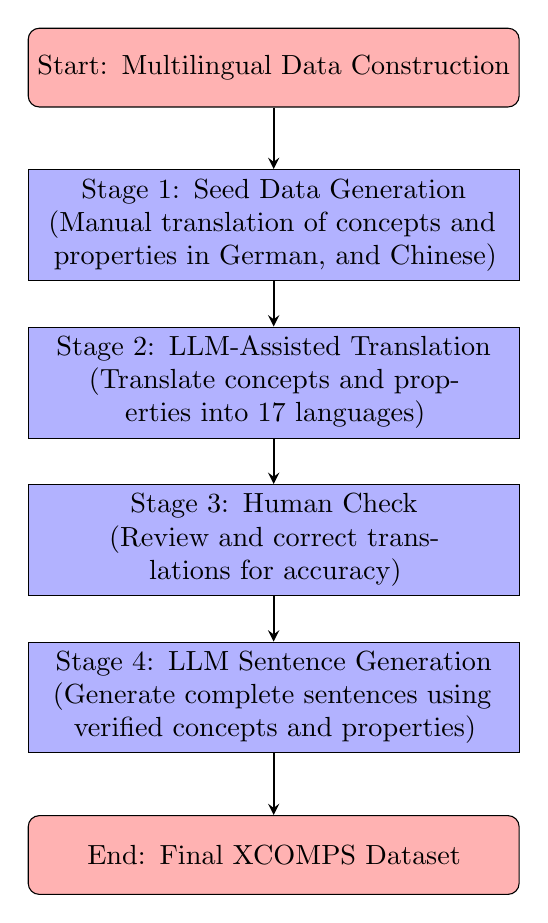
\begin{tikzpicture}[node distance=2cm]

% Nodes
\node (start) [startstop] {Start: Multilingual Data Construction};
\node (seed) [process, below of=start] {Stage 1: Seed Data Generation \\ 
(Manual translation of concepts and properties in German, and Chinese)};
\node (llmtranslate) [process, below of=seed] {Stage 2: LLM-Assisted Translation \\ 
(Translate concepts and properties into 17 languages)};
\node (humancheck) [process, below of=llmtranslate] {Stage 3: Human Check \\ 
(Review and correct translations for accuracy)};
\node (llmsentence) [process, below of=humancheck] {Stage 4: LLM Sentence Generation \\ 
(Generate complete sentences using verified concepts and properties)};
\node (end) [startstop, below of=llmsentence] {End: Final XCOMPS Dataset};

% Arrows
\draw [arrow] (start) -- (seed);
\draw [arrow] (seed) -- (llmtranslate);
\draw [arrow] (llmtranslate) -- (humancheck);
\draw [arrow] (humancheck) -- (llmsentence);
\draw [arrow] (llmsentence) -- (end);

\end{tikzpicture}}
\caption{Pipeline of LLM-Assisted Multi-Stage Benchmark Construction.}
\label{flow}
\end{figure}


\begin{figure*}
    \centering
\includegraphics[angle=270, width=0.5\linewidth]{figs/prompts_.png}
    \caption{Prompt templates of different languages used for metalinguistic prompting.}
    \label{prompt_template}
\end{figure*}

\begin{figure*}[h]
    \centering
    \includegraphics[width=1.0\linewidth]{./figs/diff.jpg}
    \caption{\small Llama-3.1 instruct-base difference and Llama-3.1 distill-base difference.}
    \label{fig:diff}
\end{figure*}


\begin{figure*}[h]
    \centering
    \includegraphics[width=0.8\linewidth]{./figs/mcomps_llama3.1_1024_scatter.pdf}
    \caption{Linear correlation among meta, direct and neuro for Llama-3.1 Base.}
    \label{fig:linear_cor_base}
\end{figure*}

\begin{figure*}[h]
    \centering
    \includegraphics[width=0.8\linewidth]{./figs/mcomps_llama3.1_chat_1024_scatter.pdf}
    \caption{Linear correlation among meta, direct and neuro for Llama-3.1 Instruct.}
    \label{fig:linear_cor_instruct}
\end{figure*}

\begin{figure*}[h]
    \centering
    \includegraphics[width=0.8\linewidth]{./figs/mcomps_deepseek_1024_scatter.pdf}
    \caption{Linear correlation among meta, direct and neuro for Llama-3.1 Distilled.}
    \label{fig:linear_cor_deepseek}
\end{figure*}

\begin{figure*}[h]
    \centering
    \includegraphics[width=1.0\linewidth]{./figs/diff_layer.jpg}
    \caption{\small Layer-wise probing perf. difference.}
    \label{fig:neuro_diff}
\end{figure*}

\begin{figure*}[h]
    \centering
    \includegraphics[width=0.8\linewidth]{./figs/peak_layer.jpg}
    \caption{Peak layer of each task and language in neurolinguistic probing.}
    \label{fig:peak_layer}
\end{figure*}

\end{document}

